\section{Interface Gráfica}\label{sec:gui}

\FloatBarrier

\begin{figure}[h]
  \centering
  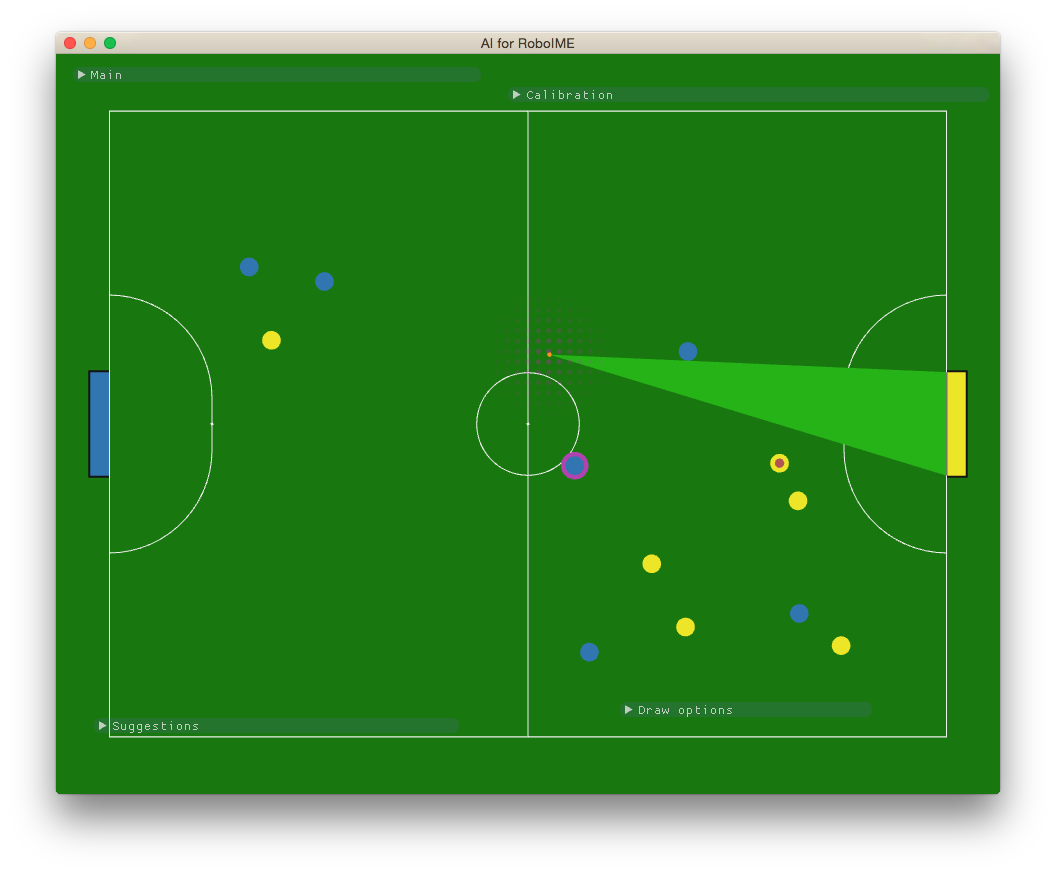
\includegraphics[width=0.8\linewidth]{gui_field}
  \caption{Aparência geral e representação do campo}\label{fig:gui_field}
\end{figure}

A ferramenta representa o estado atual do jogo desenhando o campo, os robôs e a
bola, como pode ser visto na figura~\ref{fig:gui_field}.  O campo não faz parte
do estado mas é necessário para ter uma referência visual das posições.

\begin{figure}[h]
  \centering
  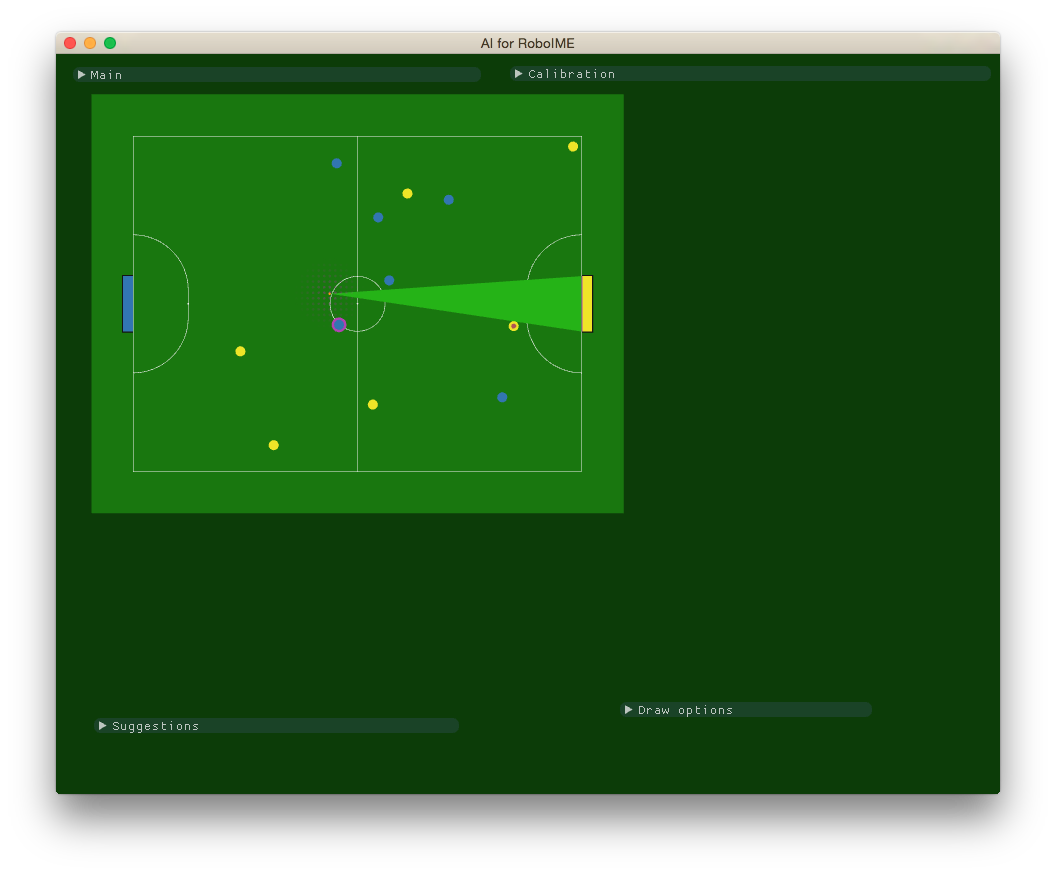
\includegraphics[width=0.4\linewidth]{gui_zoom_out}
  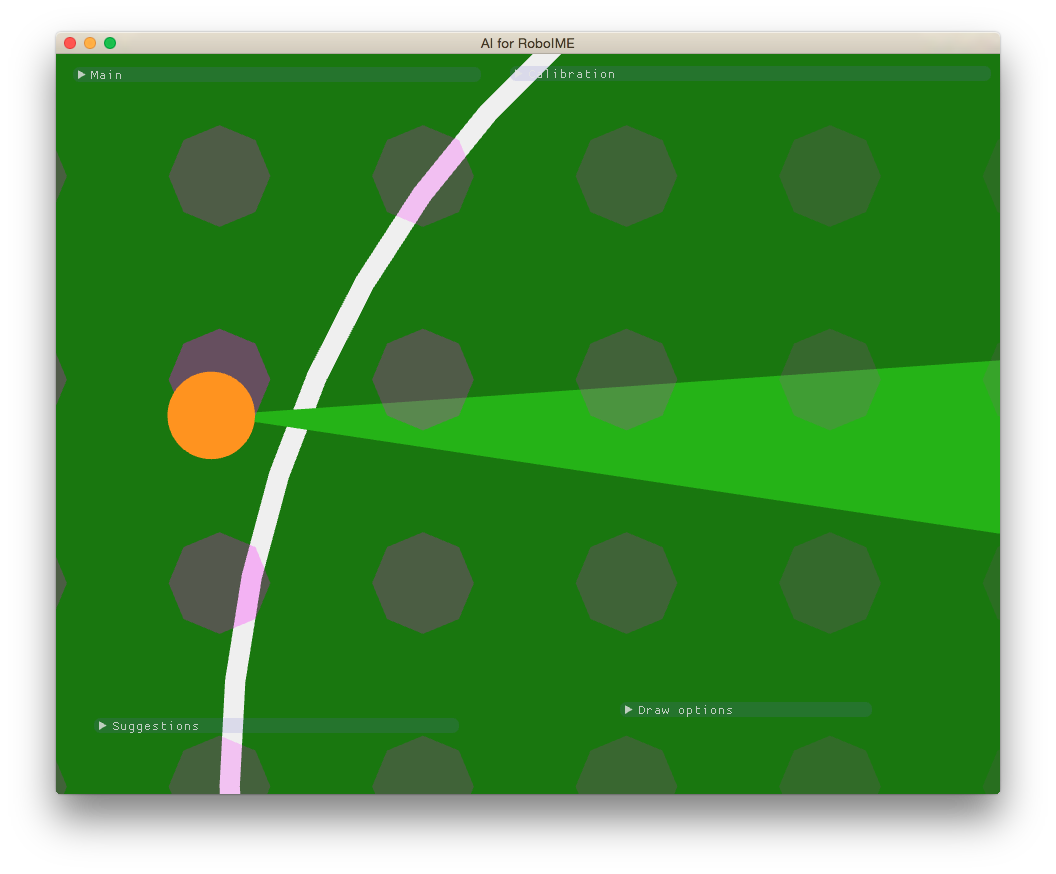
\includegraphics[width=0.4\linewidth]{gui_zoom_in}
  \caption{Zoom e arraste do campo}\label{fig:gui_zoom}
\end{figure}

Para visualizar situações com mais detalhes a ferramenta permite zoom e arraste
do campo (figura~\ref{fig:gui_zoom}).

\begin{figure}[h]
  \centering
  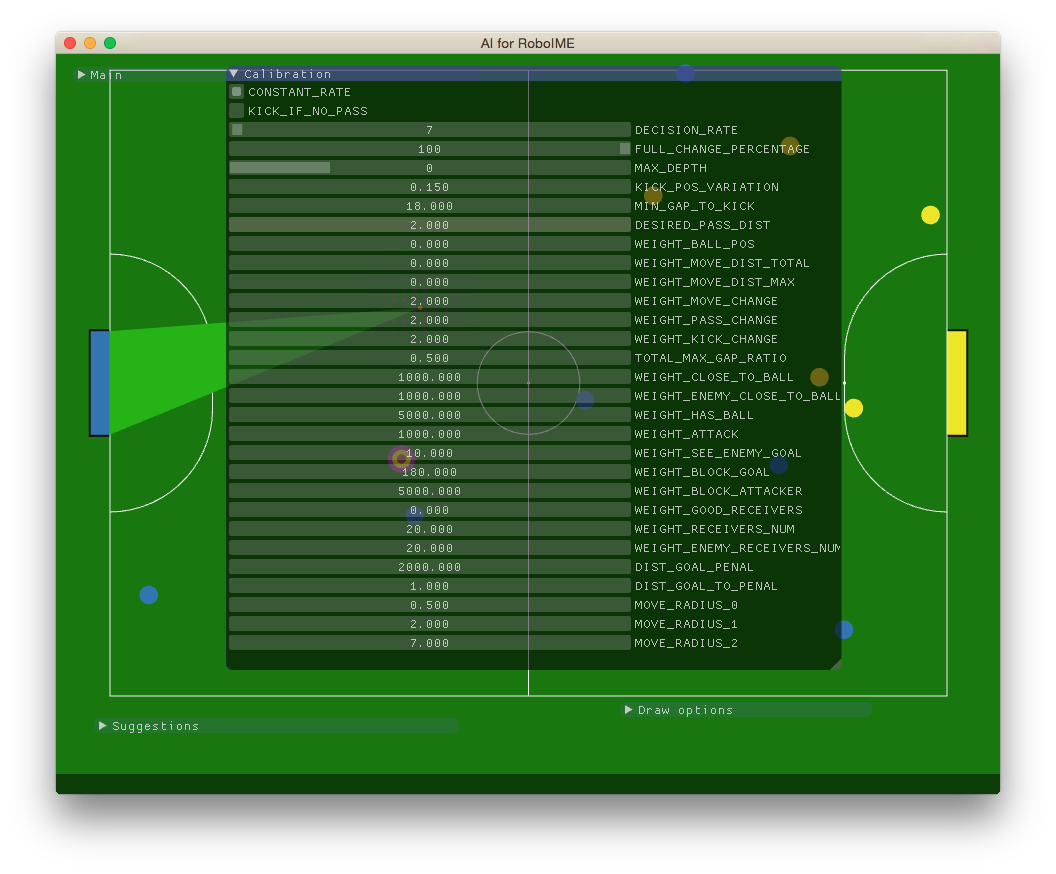
\includegraphics[width=0.8\linewidth]{gui_params}
  \caption{Parâmetros configuráveis}\label{fig:gui_params}
\end{figure}

\begin{figure}[h]
  \centering
  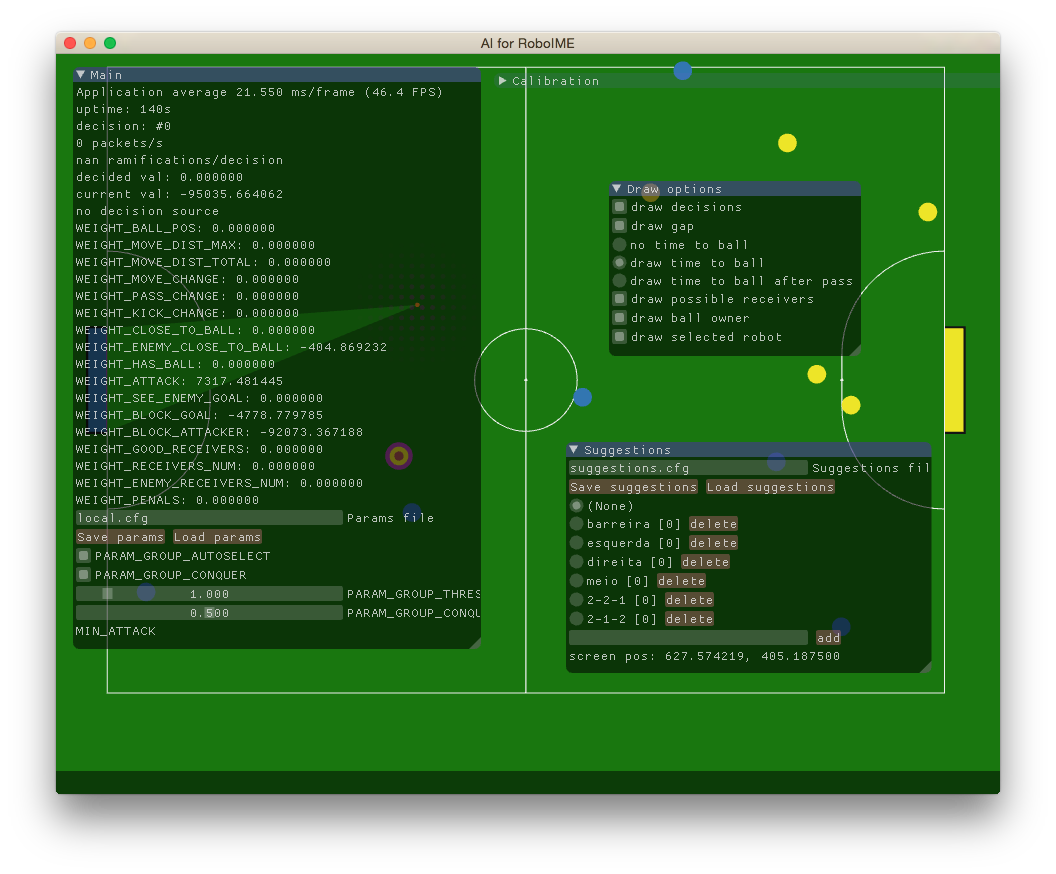
\includegraphics[width=0.8\linewidth]{gui_widgets}
  \caption{Controles}\label{fig:gui_widgets}
\end{figure}

Existem quatro abas disponíveis: \textit{Main}, \textit{Calibration},
\textit{Suggestions}, \textit{Draw options}. As abas são retráteis e
translucidas para que as mudanças de configurações possam ser observadas
facilmente.  Na figura~\ref{fig:gui_field}, por exemplo, todas as estão
minimizadas, na figura~\ref{fig:gui_params} é mostrada a aba
\textit{Calibration}, as outras três podem ser vistas na
figura~\ref{fig:gui_widgets}.

\begin{figure}[h]
  \centering
  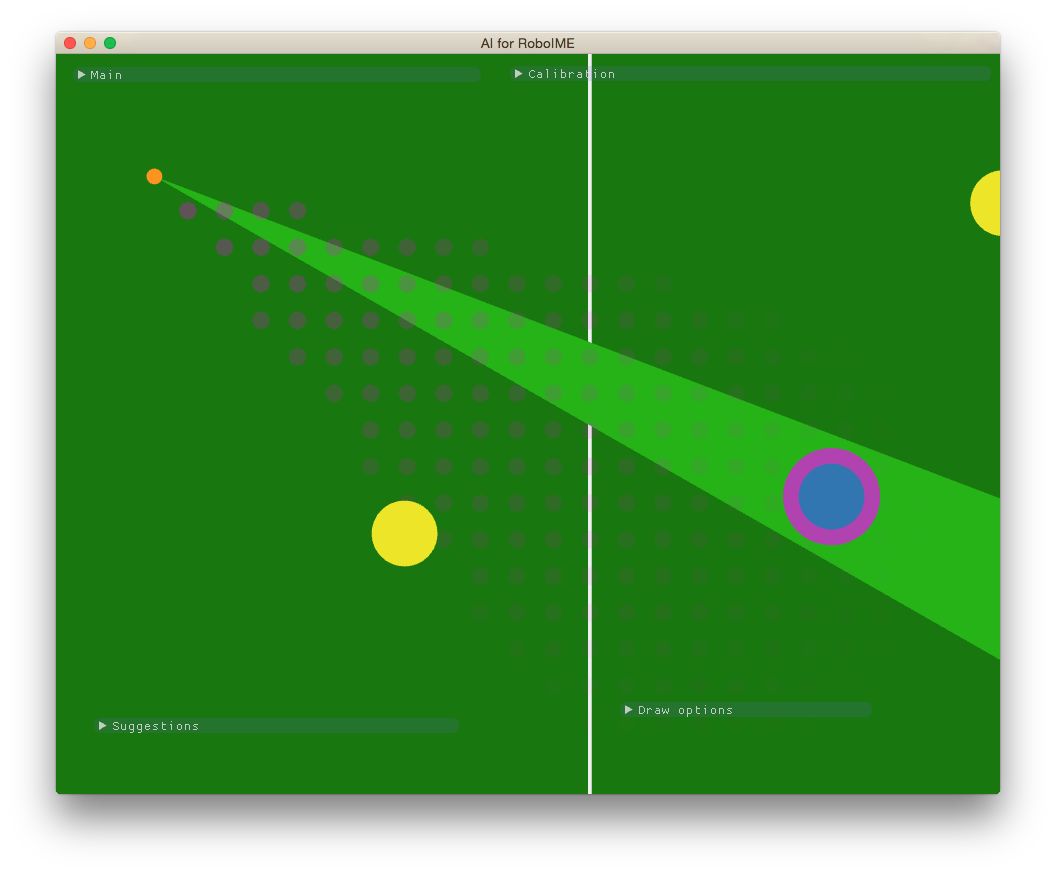
\includegraphics[width=0.4\linewidth]{gui_ball_move}
  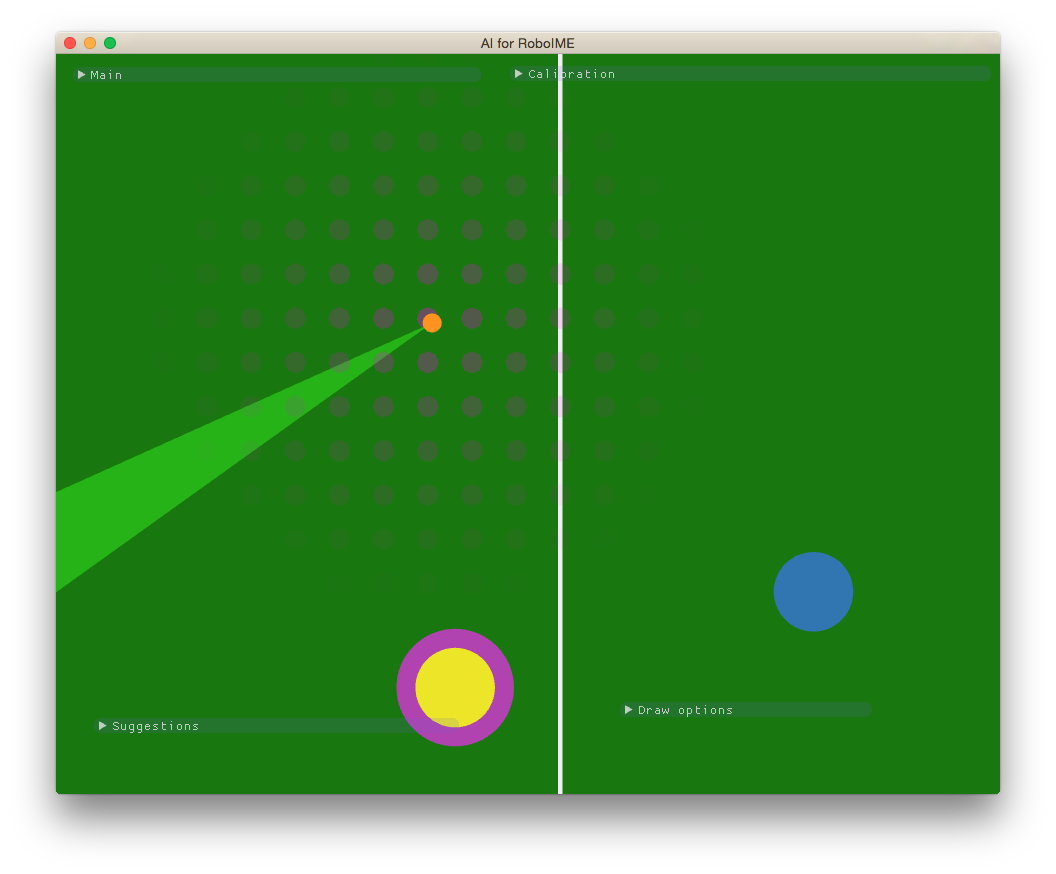
\includegraphics[width=0.4\linewidth]{gui_ball_stop}
  \caption{Representação do tempo para chegar na bola}\label{fig:gui_ball}
\end{figure}

\begin{figure}[h]
  \centering
  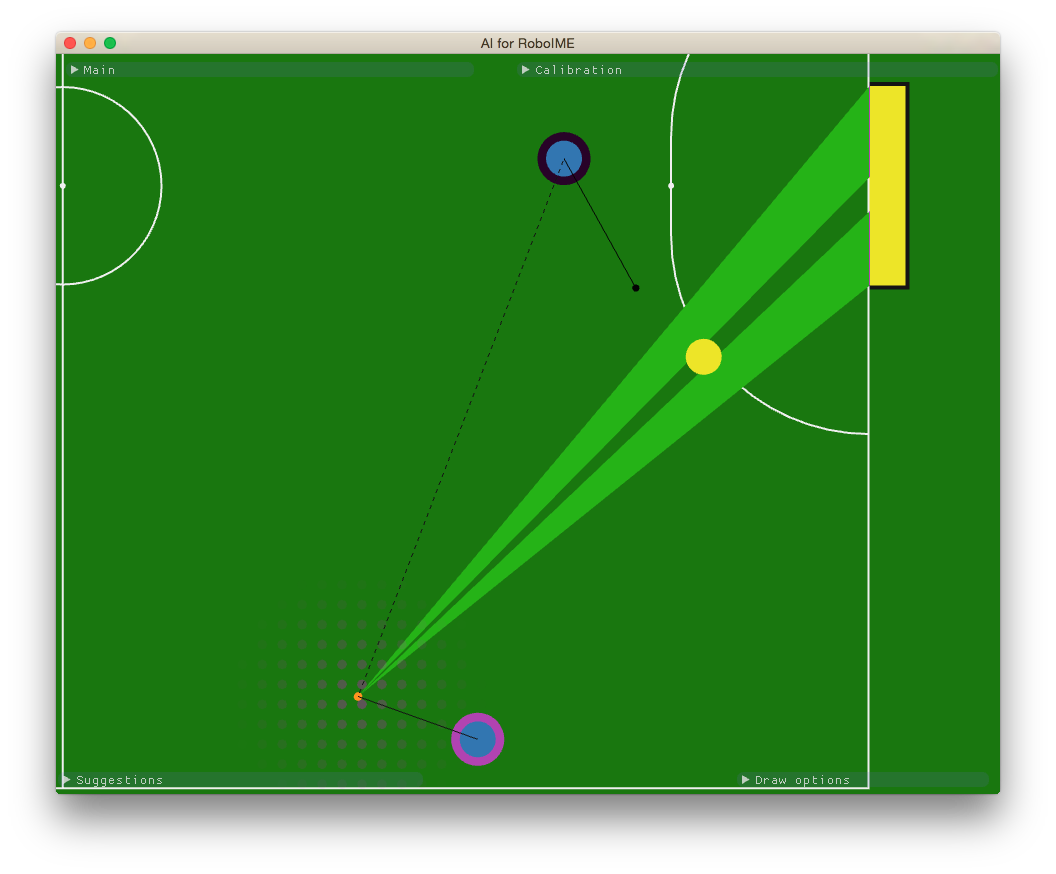
\includegraphics[width=0.8\linewidth]{gui_pass}
  \caption{Representação de ação de passe}\label{fig:gui_pass}
\end{figure}

\begin{figure}[h]
  \centering
  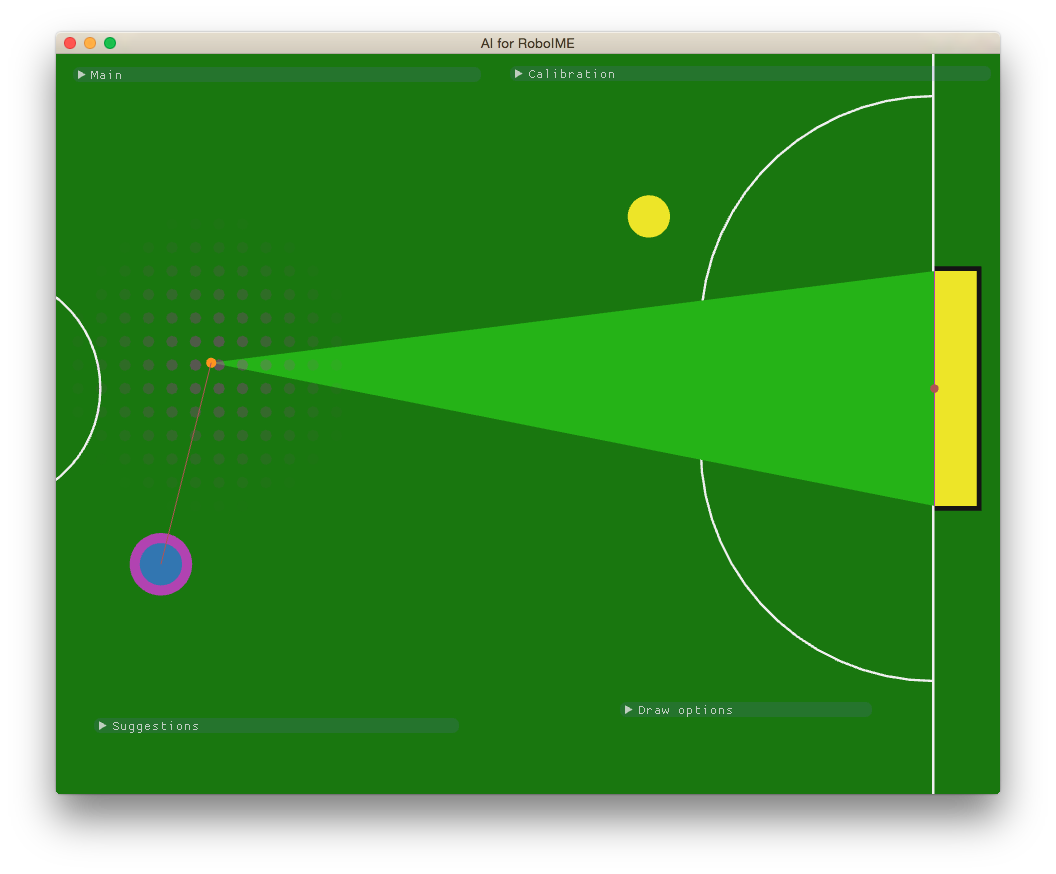
\includegraphics[width=0.8\linewidth]{gui_kick}
  \caption{Representação de ação de chute}\label{fig:gui_kick}
\end{figure}

\begin{figure}[h]
  \centering
  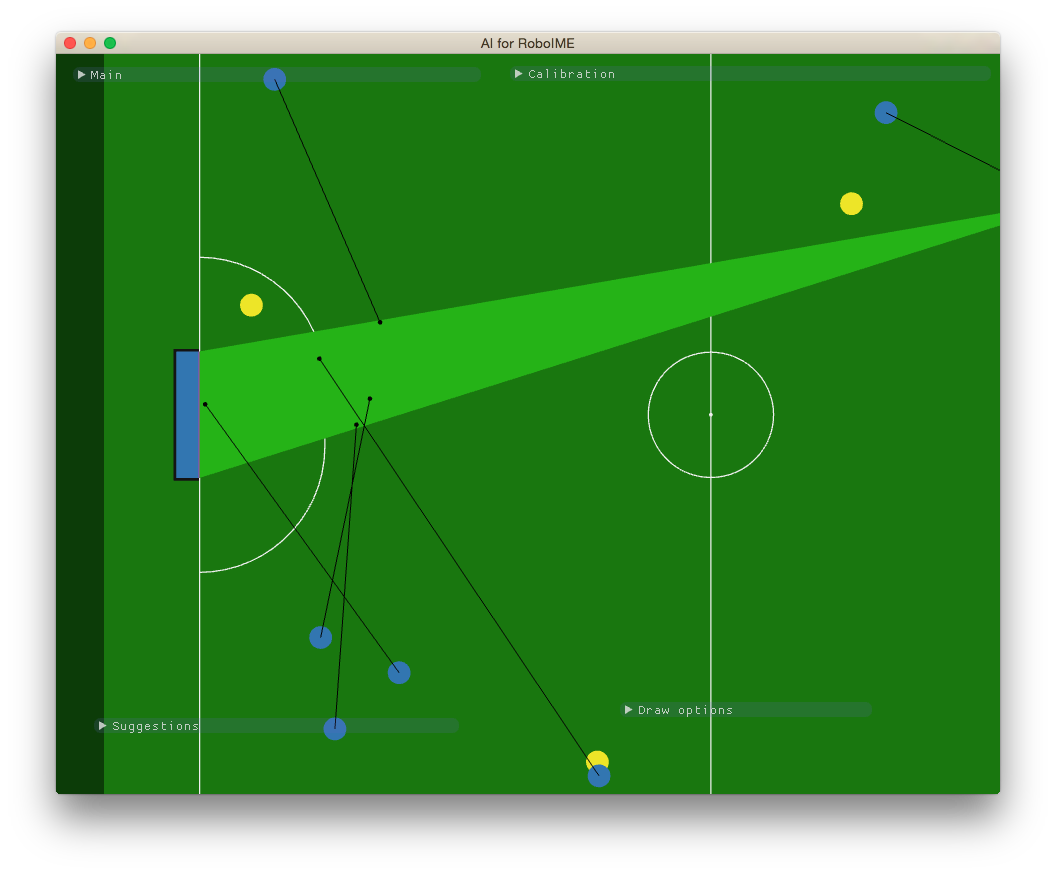
\includegraphics[width=0.8\linewidth]{gui_move}
  \caption{Representação das ações de movimentação}\label{fig:gui_move}
\end{figure}

\FloatBarrier

% vim: tw=80 et ts=2 sw=2 sts=2 ft=tex
